\documentclass[main.tex]{subfiles}
 
\begin{document}
\chapterimage{band1.jpg}
\chapter{Getting Started}

In this chapter, our aim would be to get our development setup functional, and also to get an understanding for the development tools and repositories available around ESP32.

\section{Development Overview}\index{Development Overview}

The following diagram depicts the typical developer setup for development with ESP32.
\begin{figure}[h]
    \centering
    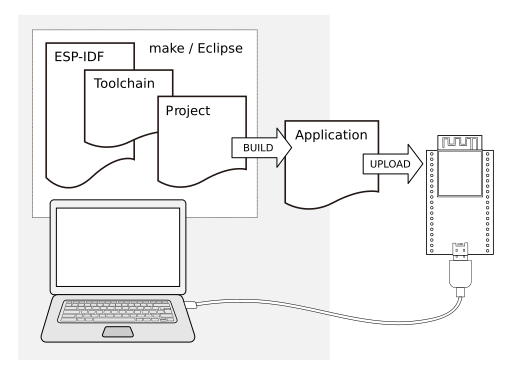
\includegraphics[scale=0.6]{../../_static/dev_setup.png}
    \caption{Typical Developer Setup}
    \label{fig:dev_setup}
\end{figure}

The PC, or the Development Host can be any of Linux, Windows or Mac. The ESP32 based development board is connected to the Development Host over a USB cable. The Development Host has the ESP-IDF (Espressif's SDK), the compiler toolchain and the code for your project. The development host builds this code and generates the executable firmware image. The tools on the Development Host then download the generated firmware image on to the development board. As the firmware executes on the development board, the logs from the firmware can be monitored from the Development Host.

\section{ESP-IDF}\index{ESP-IDF}

ESP-IDF is Espressif's IoT Development Framework. 
\begin{itemize}
    \item ESP-IDF is a collection of libraries and header files that provides the core software components that are required to build any software projects on ESP32. 
    \item ESP-IDF also provides tools and utilities that are required for typical developer and production usecases, like build, flash, debug and measure.
\end{itemize}

\subsection{Setting up IDF}\index{Setting up IDF}

Please follow the steps in this documentation for setting up IDF: \url{https://docs.espressif.com/projects/esp-idf/en/latest/get-started/index.html}. Please complete all the steps on this page.

Before proceeding, please ensure that you have setup your development host, and have built the first application as indicated in this page. Now that you have done that, let's look at some additional details about IDF.

\subsection{IDF Details}\index{IDF Details}

The IDF has a component based design.

\begin{figure}[h!]
    \centering
    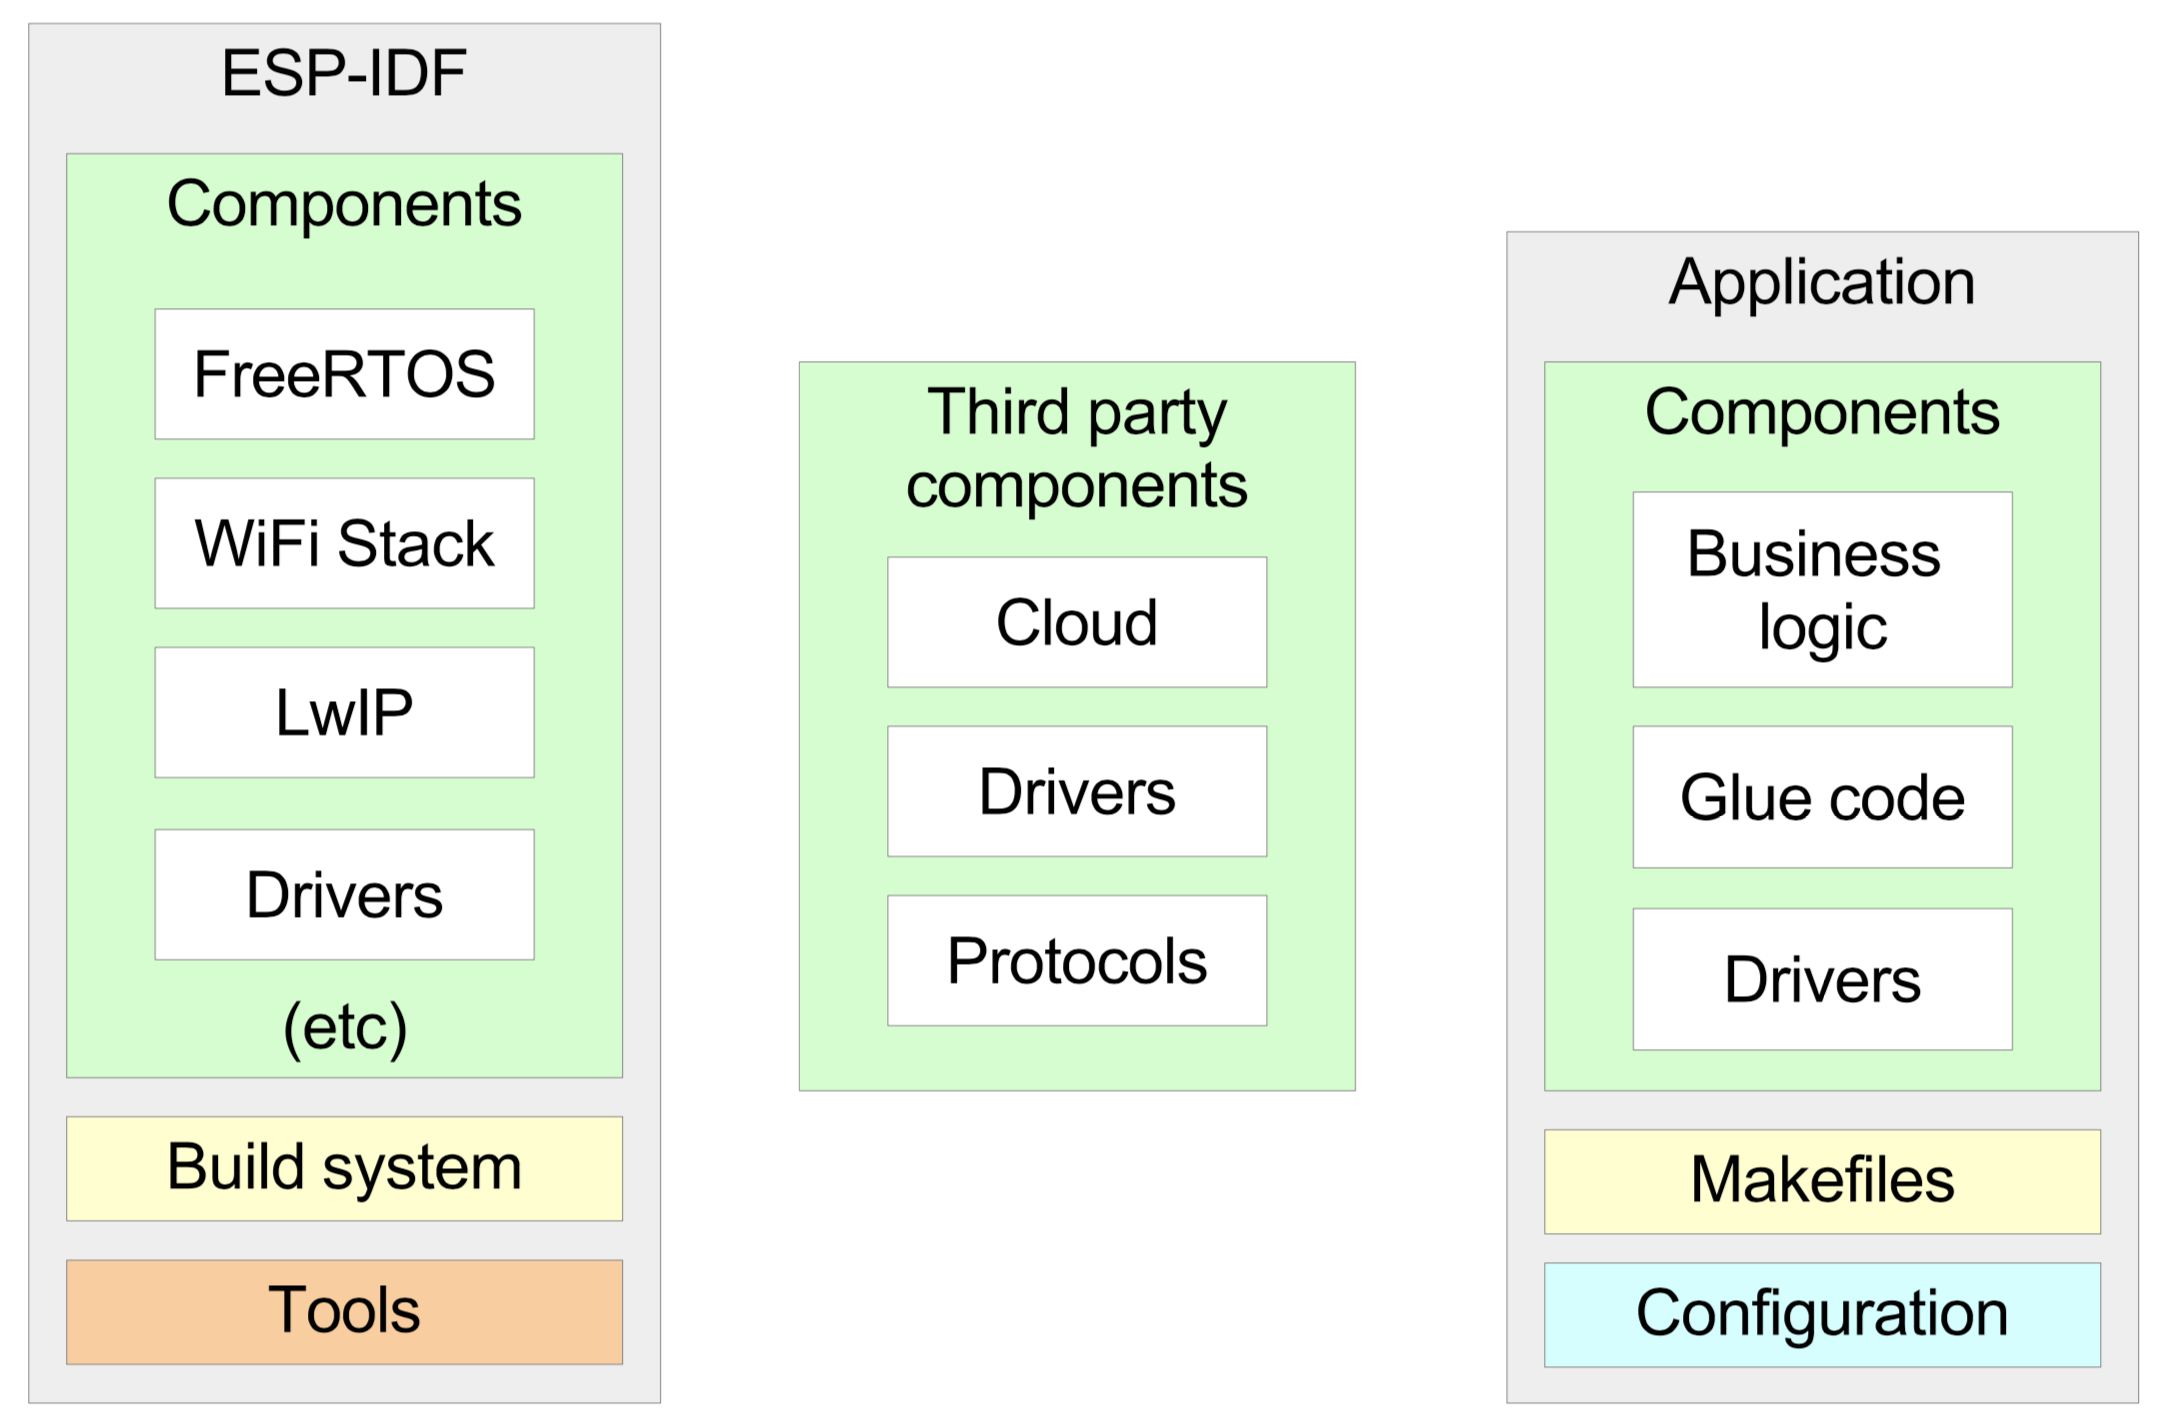
\includegraphics[width=\textwidth]{../../_static/idf_comp.png}
    \caption{Component Based Design}
    \label{fig:idf_comp_design}
\end{figure}

All the software in the IDF is available as components. The Operating System, the network stack, Wi-Fi drivers, middleware modules like the HTTP Server are all components within IDF. 

This design allows you to use your own or third-party components that are built for ESP-IDF.

A developer typically builds \textit{applications} against the IDF. The applications contain the business logic, any drivers for externally interfaced peripherals and the SDK configuration.

\begin{figure}[h!]
    \centering
    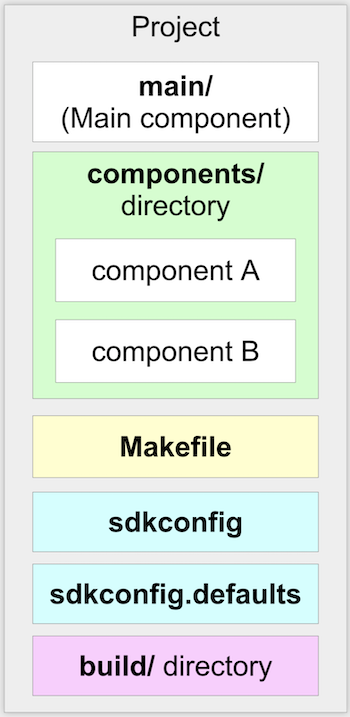
\includegraphics[scale=0.6]{../../_static/app_structure.png}
    \caption{Application's Structure}
    \label{fig:app_structure}
\end{figure}

An application must contain one \textit{main} component. This is the primary component that holds the application logic. The application may additionally include other components as may be desired.
The application's \textit{Makefile} defines the build instructions for the application. 
Additionally, an optional \textit{sdkconfig.defaults} may be placed that picks up the default SDK configuration that should be selected for this application.


\section{Getting ESP-Jumpstart}\index{Getting ESP-Jumpstart}

The ESP-Jumpstart repository contains a sequence of \textit{applications} that we will use for this exercise. These applications build with the ESP-IDF that you have setup before. Let's get started by cloning the ESP-Jumpstart git repository \url{https://github.com/espressif/esp-jumpstart}. 

\begin{verbatim}
$ git clone --recursive https://github.com/espressif/esp-jumpstart
\end{verbatim}

Since we are building a production-ready firmware here, we would want to base our development on a stable release of IDF. Currently, ESP-Jumpstart uses the stable version 3.2 of ESP-IDF. Let us first switch to that version of ESP-IDF.
\begin{verbatim}
$ cd esp-idf
$ git checkout -b release/v3.2 remotes/origin/release/v3.2
$ git submodule update --recursive
\end{verbatim}

Now we build our first, \textit{Hello World}, application from ESP-Jumpstart and flash it on to our development board. You should be already familiar with most of the steps below.

\begin{verbatim}
$ cd esp-jumpstart/1_hello_world
$ make -j8 menuconfig
$ export ESPPORT=/dev/cu.SLAB_USBTOUART   # Or the correct device name for your setup
$ export ESPBAUD=921600
$ make -j8 flash monitor
\end{verbatim}

This will then build the entire SDK and the application. Once the build is successful, it will write the generated firmware to the device.

\ksnotebox{On some development boards you may have to press a specific button configuration in order to put the development board into the 'flashing mode'. Please refer to your development board's documentation for these details. For ESP32-DevKit-C, no such button press is required, the board is automatically put into the flashing mode by the flasher utility.}

Once the flashing is successful, the device will reset and you will see the console output from this firmware.

\section{The Code}\index{The Code}
Now let's look at the code of the Hello World Application. It is only a few lines of code as shown below:
\begin{minted}{c}
#include <stdio.h>
#include "freertos/FreeRTOS.h"
#include "freertos/task.h"


void app_main()
{
    int i = 0;
    while (1) {
        printf("[%d] Hello world!\n", i);
        i++;
        vTaskDelay(5000 / portTICK_PERIOD_MS);
    }
}
\end{minted}
The code is fairly simple. A few takeaways:
\begin{itemize}
\item The app\_main() function is the application entry point. All applications begin execution at this point. This function gets called after the FreeRTOS kernel is already executing on both the cores of the ESP32. Once FreeRTOS is initialis\
ed, it forks an application thread, called the main thread, on one of the cores. The app\_main() function is called in this thread's context. The stack of the application thread can be configured through the SDK configuration.
\item C library functions like printf(), strlen(), time() can be directly called. The IDF uses the newlib C library, which is a low-footprint implementation of the C library. Most of the category of functions of the C library like stdio, stdlib, string operations, math, time/timezones, file/directory operations are supported. Support for signals, locales, wchrs is not available. In our example above, we use the printf() function for printing to the console.
\item FreeRTOS is the operating system powering both the cores. FreeRTOS (https://www.freertos.org) is a tiny kernel that provides mechanisms for task creation, inter-task communication (semaphores, message queues, mutexes), interrupts and timers. In our example above, we use the vTaskDelay function for putting the thread to sleep for 5 seconds. Details of the FreeRTOS APIs are available at: https://www.freertos.org/a00106.html
\end{itemize}

\section{Progress so far}\index{Progress so far}
Now we have the basic development setup and process in place. We can build the code into executable firmware images. We can flash these images to a connected development board, and we can monitor the console to look at debug logs and messages generated by the firmware. 

Let's now build a simple power outlet with ESP32.

\end{document}
